
\chapter{The Zeta Function of Riemann (Contd).}\label{chap14}

\setcounter{section}{8}
\section[Riemann-Von Mangoldt Formula]{Riemann-Von Mangoldt Formula \cite[p.68]{key11}}\label{chap14:sec9}
Let\pageoriginale $N(T)$ denote the number of zeros (necessarily finite) of
$\zeta(s)$ in $0 \leq \sigma \leq 1$, $0 \leq t \leq T$. Then, by what
we have proved, $N(T)$ is the number of zeros $\rho = \beta + i
\gamma$ of $\zeta(s)$, or of $\xi (s)$, for which $0< \gamma \leq T$

\setcounter{thm}{0}
\begin{thm}\label{chap14:thm1}
$N(T) = \dfrac{T}{2n} \log \left(\dfrac{T}{2 \pi}\right) - \dfrac{T}{2\pi} + O(\log
  T)$ as $T \to \infty$.
\end{thm}

\begin{proof}
Suppose first that $T$ is not equal to any $\gamma$. Also let $T
>3$. Consider the rectangle $R$ as indicated. $\xi(s)$ has $2N(T)$
zeros \textit{inside} it, and none on the boundary. Hence, by the
principle of the argument,
$$
2N(T) = \frac{1}{2\pi} [\arg \xi (s)]_R,
$$ 
where $[\arg \xi (s)]_R$ denotes the increase in $\arg\xi(s)$, as $s$
describes the boundary of $R$.
\begin{figure}[H]
\centering
\includegraphics{figures/fig14.1.eps}
\end{figure}

Now
$$
[\arg \xi (s)]_R = \left[\arg\frac{1}{2} s (s-1)\right]_R + [\arg\eta (s)]_R,
$$
where $\eta(s) = \pi^{-s/2} \Gamma (s/2)\zeta(s)$. Here
$$
\left[\arg \frac{1}{2}s(s-1)\right]_R = 4 \pi,
$$
and $\eta(s)$ has the properties: $\eta(s) = \eta(1-s)$, and
$\eta(\sigma \pm ti)$ are conjugates.\pageoriginale Hence
$$
[\arg \eta(s)]_R = 4 [\arg \eta(s)]_{ABC}
$$
Hence
\begin{align}
\pi N(T) = \pi + \arg [\pi^{-s/2}] & + [\arg \Gamma(s/2)]_{ABC} + [\arg \zeta(s)]_{ABC}\label{c14:eq9.1}
\end{align}
Now 
\begin{equation}
[\arg \pi^{-s/2}]_{ABC} = \left[-\frac{t}{2} \log \pi \right]_{ABC} =
- \frac{T}{2} \log \pi. \label{c14:eq9.2}
\end{equation}
Next, since $\Gamma (z+\alpha) = (z+\alpha -\frac{1}{2}) \log z -z +
\frac{1}{2} \log 2 \pi + O(|z|^{-1})$  as $|z| \to \infty$, in any
angle $|\arg z| \leq \pi - \epsilon <\pi$, we have
\eject
\begin{align}
&\left[\arg\Gamma\left(\frac{1}{2}\right) \right]_{ABC} = \left[\im \log \Gamma
  (s/2) \right]_{ABC}\notag\\
&\quad =\im \log \Gamma \left(\frac{1}{4} + \frac{1}{2} i T \right)   - \im \log \Gamma
(1)\notag\\
&\quad = \im \left\{ \left(-\frac{1}{4} + \frac{1}{2} i T \right) \log \left(\frac{1}{2} i T \right)
- \frac{1}{2} i T + \frac{1}{2} \log 2 \pi + O (T^{-1})\right\}\notag\\
&\quad = \frac{1}{2} T \log \left(\frac{1}{2}T \right) - \frac{1}{8} \pi -\frac{T}{2} +
O \left(T^{-1} \right), \text{ as } T \to \infty\label{c14:eq9.3}
\end{align}

Using \eqref{c14:eq9.2} and \eqref{c14:eq9.3} in \eqref{c14:eq9.1}, we get
\begin{equation}
N(T) = \frac{T}{2\pi} \log \left(\frac{T}{2\pi}\right) - \frac{T}{2\pi} +
\frac{7}{8} + \frac{1}{\pi} [\arg \zeta(s)]_{ABC} + 0 \left(
\frac{1}{T}\right) \label{c14:eq9.4}
\end{equation}

Consider the broken line ABC exclusive of the end-points $A$ and
$C$. If $m$ is the number of distinct points $s'$ on ABC at which $\re
\zeta (s) =0$, then 
\begin{equation}
[\arg \zeta(s)]_{ABC} \leq (m+1) \pi,\label{c14:eq9.5}
\end{equation}\pageoriginale
since $\arg \zeta(s)$ cannot vary by more than $\pi$ (since $\re
\zeta$ does not change sign here) on any one of the $m+1$ segments
into which ABC is divided by the point $s'$.

Now no point $s'$ can be on AB, for 
\begin{equation}
\re \zeta (2+iT) \geq 1 - \sum\limits^\infty_2 \frac{1}{n^2} > 1 -
\frac{1}{2^2}  - \int\limits^\infty_2 \frac{du}{u^2} = \frac{1}{4}.
\label{c14:eq9.6}
\end{equation}
Thus $m$ is the number of distinct points $\sigma$ of $\frac{1}{2} <
\sigma < 2$ at which $\re \zeta (\sigma + i T) =0$, i.e. the number of
distinct zeros of 
$$
g(s) = \frac{1}{2} \{\zeta (s + iT) + \zeta(s-iT)\}
$$
on the real axis for which $\frac{1}{2} <\sigma < 2$, because
$g(\sigma) = \re \zeta(\sigma + iT)$ for real $\sigma$, since $\zeta
(\sigma \pm iT)$ are conjugate.

Now since $g(s)$ is regular except for $s=1\pm iT$, $m$ must be
finite, and we can get an upper bound for $m$ by using a theorem
proved earlier. 

Consider the two circles: $|s - 2 | \leq \dfrac{7}{4}$, $|s-2| \leq
\dfrac{3}{2}$. Since $T>3$, $g(s)$ is regular in the larger circle. At
all points $s$ of {\em this} circle, we have
$$
\sigma \geq \frac{1}{4}, \quad 1 < |t \pm T| < 2 + T.
$$
Hence, by an appeal to the other of $\zeta(s)$ obtained in the \ref{chap12}th
Lecture (with $\delta=\frac{1}{4}$), we get
\begin{align*}
|g(s)| & < \frac{1}{2} c_1 \left(|t+T|^{3/4} + |t-T|^{3/4}\right)\\
& < c_1 (T+2)^{3/4},
\end{align*}
on the larger circle. At the centre, we have 
$$
g(2) = \re \zeta(2+iT)  > \frac{1}{4} \text{ by (9.6)}
$$
Hence,\pageoriginale by using the theorem (given in the Appendix), we
get
$$
\left(\frac{7}{6} \right)^m <\frac{c_1(T+2)^{3/4}}{\frac{1}{4}} < T , \text{ for }
T > T_0 \geq 3.
$$

Thus 
$$
m < c_2 \log T, \text{ for }T > T_0.
$$
Substituting this into \eqref{c14:eq9.5} and \eqref{c14:eq9.4} we get
$$
\left|N(T) -\frac{T}{2\pi} \log \left(\frac{T}{2\pi}\right) + \frac{T}{2\pi}
\right| \leq c_3 \log T, \quad T > T_0,
$$
provided that $T \neq \gamma$ for any `$\gamma$'. The last restriction
may be removed by first taking $T'$ larger than $T$ and distinct from
the $\gamma's$ and then letting $T'\to T +0$.
\end{proof}

\begin{remarks*}
The above theorem was stated by Riemann but proved by Von Mangoldt in
1894. The proof given here is due to Backlund (1914).
\end{remarks*}

\setcounter{corollary}{0}
\begin{corollary}\label{chap14:coro1}
If $h>0$ (fixed), then 
$$
N(T +h) - N(T) = O (\log T), \text{ as } T \to \infty
$$
\end{corollary}

\begin{proof}
If we write
$$
f(t) = \frac{t}{2\pi} \log \frac{t}{2\pi} - \frac{t}{2\pi},
$$
we get
$$
f(t+h) - f(t) = h f'(t+\theta h), 0 < \theta < 1,
$$
where $f'(t) = \dfrac{1}{2\pi} \log \dfrac{t}{2\pi}$. Now use the Theorem.
\end{proof}

\begin{corollary}\label{chap14:coro2}
$$
S \equiv \sum\limits_{0 \leq \gamma \leq T} \frac{1}{\gamma} =
O(\log^2 T); S' \equiv \sum\limits_{\gamma >T} \frac{1}{\gamma^2} =
O \left(\frac{\log T}{T} \right)
$$
(summed over all zeros $\rho$ whose imaginary parts $\gamma$ satisfy
the given conditions).

%raghu gv 117

Let\pageoriginale
\begin{align*}
s_m & = \sum \frac{1}{\gamma}, \quad m < \gamma \leq m+1, \text{ and }\\
s'_m & = \sum \frac{1}{\gamma^2},  \quad m < \gamma\leq m+1.
\end{align*}

Then
$$
S \leq \sum\limits^{[T]}_{m=0} s_m, \quad S' \leq \sum\limits^\infty_{m=[T]}
s'_m 
$$

If $m \geq 1$, the number of terms in $s_m$ (or $s'_m$) is 
$$
N(m+1) - N (m) = \nu_m, \text{ say}.
$$
By Corollary \ref{chap14:coro1}, $\nu_m =O(\log m)$ as $m \to \infty$; and 
$$
s_m \leq \frac{\nu_m}{m}, \quad s_m \leq \frac{\nu_m}{m^2}
$$
Hence, as $T \to \infty$,
\begin{align*}
S & = O(1) + O \left( \sum^{[T]}_{2} \frac{\log m}{m}\right) =
O(\log^2 T)\\
S' & = O \left(\sum\limits^\infty_{[T]} \frac{\log m}{m^2} \right) = O
\left(\frac{\log T}{T} \right)
 \end{align*}
\end{corollary}

\begin{corollary}\label{chap14:coro3}
If the zeros `$\rho$' for which $\gamma >0$ are arranged as a sequence
$\rho_n = \beta_n + i \gamma_n$, so that $\gamma_{n+1} \geq \gamma_n$,
then 
$$
|\rho_n| \sim \gamma_n \sim \frac{2\pi n}{\log n} , \text{ as } n \to
\infty 
$$
\end{corollary}

\begin{proof}
Since $N(\gamma_n -1) < n \leq N (\gamma_n +1)$, and
\begin{align*}
2 \pi N (\gamma_n \pm 1) & \sim (\gamma_n \pm 1) \log (\gamma_n \pm
1)\\
& \sim \gamma_n \log \gamma_n,
\end{align*}\pageoriginale
we have first
$$
2 \pi n \sim \gamma_n\log \gamma_n
$$
whence
$$
\log n \sim \log \gamma_n,
$$
and \quad $\gamma_n \sim \dfrac{2\pi n}{\log \gamma_n} \sim
\dfrac{2\pi n}{\log n}$

\medskip

And \quad $\gamma_n \leq |\rho_n| < \gamma_n + 1$.
\end{proof}

\begin{remarks*}
\begin{itemize}
\item[{\rm (i)}]  The main theorem proves incidentally the existence
  of an infinity of complex zeros of $\zeta(s)$, {\em without} the use of
  the theory of entire functions.

\item[{\rm (ii)}] We see from corollary \ref{chap14:coro3} that 
$$
\sum \frac{1}{|\rho|(\log |\rho|)^\alpha}
$$
converges for $\alpha >2$ and diverges for $\alpha \leq 2$.

\item[{\rm (iii)}] Corollary \ref{chap14:coro1} may be obtained directly by applying
  the theorem (on the number of zeros) to $\zeta(s)$ and to two
  circles with centre at $c+iT$ and passing through $\frac{1}{2}+ (T
  + 2h)i$, $\frac{1}{2}+(T+h)i$ respectively, where $c=c(h)$ is
  sufficiently large, and using the symmetry about $\sigma =1/2$

\item[{\rm (iv)}] If $N_0(T)$ denotes the number of complex zeros of
  $\zeta(s)$ with real part $\frac{1}{2}$ and imaginary part between
  $0$ and $T$, then Hardy and Littlewood proved that $N_0(T)>c T$ in
  comparison with $N(T) \sim \dfrac{1}{2\pi} T \log$ A. Selberg has
  shown, however, that $N_0 (T)>c T \log T$.
\end{itemize}
\end{remarks*}


\begin{center}
{\bf Appendix}
\end{center}

\begin{theorem*}
Let\pageoriginale $f(z)$ be regular in $|z-z_0| \leq R$ and have $n$
zeros (at least) in $|z-z_0| \leq r < R$. Then, if $f(z_0) \neq 0$.
$$
\left(\frac{R}{r}\right)^n \leq \frac{M}{|f(z_0)|},
$$
where $M = \max\limits_{|z-z_0|=R} |f(z)|$
\end{theorem*}

\begin{proof}
Multiple zeros are counted according to multiplicity. Suppose $z_0=0$
(for otherwise put $z=z_0+z'$). Let $a_1, \ldots, a_n$ be the zeros of
$f(z)$ in $|z|\leq r$. 

Then 
$$
f(z) = \varphi(z) \prod\limits^n_{\nu=1}
\dfrac{R(z-a_\nu)}{R^2 - \overline{\lambda}_\nu z}
$$
 where $a_\nu$, $\overline{a_\nu}$ are conjugates and $\varphi$ is regular in $|z|
\leq R$. On $|z| = R$, each factor has modulus 1; hence
$$
|\varphi(z)| = |f(z)| \leq M \text{ on }|z|=R
$$
Since $\varphi$ is regular in $|z| \leq R$, we have
$$
|\varphi (0)| \leq M
$$

Hence \quad $|f(0)| = | \varphi(0)| \prod\limits^n_{\nu=1}
\dfrac{|a_\nu|}{R} \leq M \left(\frac{r}{R}\right)^n$ and $f(0) \neq
0$, hence the result.
\end{proof}

\begin{theorem*}
If $f$ is analytic inside and on $C$ and $N$ is the number of zero
inside $C$, then
\begin{gather*}
\frac{1}{2\pi i} \int\limits_C \dfrac{f'(z)}{f(z)} dz = N\\
= \Delta_c \log \{f(z)\}
\end{gather*}
so that
$$
N = \frac{1}{2\pi} \Delta_c \arg f(z).
$$
\end{theorem*}
